%%%%%%%%%%%%%%%%%%%%%%%%%%%%%%%%%%%%%%%%%%%%%%%%%%%%%%%%%%%%%%%%%%%%%%%%
%     LaTeX source code to approximate a NIST Technical report
%	  Instructions for authors: tinyurl.com/techpubsnist
%	DOI watermark will be added on final PDF
% 	Developed by K. Miller, kmm5@nist.gov
%	Last updated: 10-Oct-2017
%%%%%%%%%%%%%%%%%%%%%%%%%%%%%%%%%%%%%%%%%%%%%%%%%%%%%%%%%%%%%%%%%%%
\documentclass[12pt]{article}
\usepackage{amsmath}
\usepackage{amsfonts}   % if you want the fonts
\usepackage{amssymb}    % if you want extra symbols
\usepackage{graphicx}   % need for figures
\usepackage{xcolor}
\usepackage{bm}
\usepackage{secdot}		
\usepackage{mathptmx}
\usepackage{multirow}
\usepackage{float}
\usepackage[utf8]{inputenc}
\usepackage{textcomp}
\usepackage[hang,flushmargin,bottom]{footmisc} % footnote format
\usepackage{placeins}
\newcommand{\ct}{\tt\small}

\usepackage{titlesec}
\titleformat{\section}{\normalsize\bfseries}{\thesection.}{1em}{}	% required for heading numbering style
\titleformat*{\subsection}{\normalsize\bfseries}

\usepackage{tocloft}	% change typeset, titles, and format list of appendices/figures/tables
\renewcommand{\cftdot}{}	
\renewcommand{\contentsname}{Table of Contents}
\renewcommand{\cftpartleader}{\cftdotfill{\cftdotsep}} % for parts
\renewcommand{\cftsecleader}{\cftdotfill{\cftdotsep}}
\renewcommand\cftbeforesecskip{\setlength{4pt}{}}
\addtolength{\cftfignumwidth}{1em}
\renewcommand{\cftfigpresnum}{\figurename\ }
\addtolength{\cfttabnumwidth}{1em}
\renewcommand{\cfttabpresnum}{\tablename\ }
\setlength{\cfttabindent}{0in}    %% adjust as you like
\setlength{\cftfigindent}{0in}

\usepackage{enumitem}         % to control spacing between bullets/numbered lists

\usepackage[numbers,sort&compress]{natbib} % format bibliography
\renewcommand{\bibsection}{}
\setlength{\bibsep}{0.0pt}

\usepackage[hidelinks]{hyperref} % hyperref package & removing outline from links

\usepackage{epstopdf} % converting EPS figure files to PDF

\usepackage{fancyhdr, lastpage}	% formatting document, calculating number of pages, formatting headers
\setlength{\topmargin}{-0.5in}
\setlength{\headheight}{39pt}
\setlength{\oddsidemargin}{0.25in}
\setlength{\evensidemargin}{0.25in}
\setlength{\textwidth}{6.0in}
\setlength{\textheight}{8.5in}

\usepackage{caption} % required for Figure labels
\captionsetup{font=small,labelfont=bf,figurename=Fig.,labelsep=period,justification=raggedright}

%%%%%%%%%%% !!!!!! REQUIRED - FILL OUT METADATA HERE !!!!!!!! %%%%%%%%%%%%%%
%  	Report Number - fill in Report Number sent to you (see info below)
%   DOI Statement - fill in DOI sent to you
%   Month Year - fill in Month and Year of Publication
%%%%%%%%%%%%%%%%%%%%%%%%%%%%%%%%%%%%%%%%%%%%%%%%%%%%%%%%%%%%%%%%%%%%%%%%%%%%%%%%%%%%%%
\newcommand{\pubnumber}{XXXX}
\newcommand{\DOI}{https://doi.org/10.6028/NIST.TN.XXXX}
\newcommand{\monthyear}{November 2023}
%%%%%%%%%%%%%%%%%%%%%%%%%%%%%%%%%%%%%%%%%%%%%%%%%%%%%%%%%%%%%%%%%%%%
%   	BEGIN DOCUMENT
%%%%%%%%%%%%%%%%%%%%%%%%%%%%%%%%%%%%%%%%%%%%%%%%%%%%%%%%%%%%%%%%%%%%
\begin{document}
	\urlstyle{rm} % Format style of \url
	
%%%%%%%%%%%%%%%%%%%%%%%%%%%%%%%%%%%%%%%%%%%%%%%%%%%%%%%%%%%%%%%%%%%%
%   Cover Page is REQUIRED and must contain the information
%	displayed here, at a minimum. Additional artwork may be included
%	(e.g., official project/conference logo, etc.).
%	Pub Number automated based on metadata
%%%%%%%%%%%%%%%%%%%%%%%%%%%%%%%%%%%%%%%%%%%%%%%%%%%%%%%%%%%%%%%%%%%%
	\begin{titlepage}
		\begin{flushright}
%%%%%%%%%%%%%%%%%%%%%%%%%%%%%%%%%%%%%%%%%%%%%%%%%%%%%%%%%%%%%%%%%%%%
% 	Automated based on metadata - delete if not applicable
%%%%%%%%%%%%%%%%%%%%%%%%%%%%%%%%%%%%%%%%%%%%%%%%%%%%%%%%%%%%%%%%%%%%
\LARGE{\textbf{NIST Technical Note df \pubnumber}}\\
\vfill
%%%%%%%%%%%%%%%%%%%%%%%%%%%%%%%%%%%%%%%%%%%%%%%%%%%%%%%%%%%%%%%%%%%%
%	Title
%%%%%%%%%%%%%%%%%%%%%%%%%%%%%%%%%%%%%%%%%%%%%%%%%%%%%%%%%%%%%%%%%%%%
\Huge{\textbf{Circuit \textbf{B}reaker Fires in \textbf{E}lectrical \textbf{C}abinets (BECCA Fire)}}\\
\vfill
%%%%%%%%%%%%%%%%%%%%%%%%%%%%%%%%%%%%%%%%%%%%%%%%%%%%%%%%%%%%%%%%%%%%
%	Authors - add complete list of authors, affiliations will be
%   added on title page
%%%%%%%%%%%%%%%%%%%%%%%%%%%%%%%%%%%%%%%%%%%%%%%%%%%%%%%%%%%%%%%%%%%%
\large Kevin McGrattan \\ Isaac Leventon \\
\vfill
%%%%%%%%%%%%%%%%%%%%%%%%%%%%%%%%%%%%%%%%%%%%%%%%%%%%%%%%%%%%%%%%%%%%
%	The DOI is automated based on metadata.	
%%%%%%%%%%%%%%%%%%%%%%%%%%%%%%%%%%%%%%%%%%%%%%%%%%%%%%%%%%%%%%%%%%%%
\normalsize This publication is available free of charge from:\\
\DOI\\
\vfill
%%%%%%%%%%%%%%%%%%%%%%%%%%%%%%%%%%%%%%%%%%%%%%%%%%%%%%%%%%%%%%%%%%%%
%	NIST LOGO - keep as-is
%%%%%%%%%%%%%%%%%%%%%%%%%%%%%%%%%%%%%%%%%%%%%%%%%%%%%%%%%%%%%%%%%%%%


\includegraphics[width=0.5\linewidth]{../FIGURES/NRC_logo} %\hfill

\vspace{0.5in}


\includegraphics[width=0.3\linewidth]{../FIGURES/NIST-logo}\\


\end{flushright}
\end{titlepage}
\begin{titlepage}
%%%%%%%%%%%%%%%%%%%%%%%%%%%%%%%%%%%%%%%%%%%%%%%%%%%%%%%%%%%%%%%%%%%%
%	Title Page is REQUIRED
%%%%%%%%%%%%%%%%%%%%%%%%%%%%%%%%%%%%%%%%%%%%%%%%%%%%%%%%%%%%%%%%%%%%
\begin{flushright}
%%%%%%%%%%%%%%%%%%%%%%%%%%%%%%%%%%%%%%%%%%%%%%%%%%%%%%%%%%%%%%%%%%%%
%   Publication Series & Number - automated
%%%%%%%%%%%%%%%%%%%%%%%%%%%%%%%%%%%%%%%%%%%%%%%%%%%%%%%%%%%%%%%%%%%%
\LARGE{\textbf{NIST Technical Note \pubnumber}}\\
\vfill
%%%%%%%%%%%%%%%%%%%%%%%%%%%%%%%%%%%%%%%%%%%%%%%%%%%%%%%%%%%%%%%%%%%%
%	Title
%%%%%%%%%%%%%%%%%%%%%%%%%%%%%%%%%%%%%%%%%%%%%%%%%%%%%%%%%%%%%%%%%%%%
\Huge{\textbf{Circuit \textbf{B}reaker Fires in \textbf{E}lectrical \textbf{C}abinets (BECCA Fire)}}\\
\vfill
%%%%%%%%%%%%%%%%%%%%%%%%%%%%%%%%%%%%%%%%%%%%%%%%%%%%%%%%%%%%%%%%%%%%
%	Author Order and Grouping. Always identify the primary author/creator first (s/he does not have to be a NIST author). For publications with multiple authors, group authors by their organizational affiliation. The organizational groupings and the names within each grouping should generally be ordered by decreasing level of contribution.
%	For non-NIST authors, list their city and state below their organization name.
%	For NIST authors, include the Division and Laboratory names (but do not include their city and state).
%%%%%%%%%%%%%%%%%%%%%%%%%%%%%%%%%%%%%%%%%%%%%%%%%%%%%%%%%%%%%%%%%%%%
\normalsize Kevin McGrattan \\ Isaac Leventon \\
\textit{Fire Research Division}\\
\textit{Engineering Laboratory}\\
\vfill
%%%%%%%%%%%%%%%%%%%%%%%%%%%%%%%%%%%%%%%%%%%%%%%%%%%%%%%%%%%%%%%%%%%%
%   DOI Statement - automated
%%%%%%%%%%%%%%%%%%%%%%%%%%%%%%%%%%%%%%%%%%%%%%%%%%%%%%%%%%%%%%%%%%%%
\normalsize This publication is available free of charge from:\\
\DOI\\
\vfill
%%%%%%%%%%%%%%%%%%%%%%%%%%%%%%%%%%%%%%%%%%%%%%%%%%%%%%%%%%%%%%%%%%%%
%   Date - Month and Year - automated
%%%%%%%%%%%%%%%%%%%%%%%%%%%%%%%%%%%%%%%%%%%%%%%%%%%%%%%%%%%%%%%%%%%%
\normalsize \monthyear
\vfill
%%%%%%%%%%%%%%%%%%%%%%%%%%%%%%%%%%%%%%%%%%%%%%%%%%%%%%%%%%%%%%%%%%%%
%  Department of Commerce LOGO - leave as-is
%%%%%%%%%%%%%%%%%%%%%%%%%%%%%%%%%%%%%%%%%%%%%%%%%%%%%%%%%%%%%%%%%%%%	


\includegraphics[width=0.4\linewidth]{../FIGURES/NRC_logo}  \hspace{0.5in}

\includegraphics[width=0.18\linewidth]{../FIGURES/DoC-logo}\\
\vfill
%%%%%%%%%%%%%%%%%%%%%%%%%%%%%%%%%%%%%%%%%%%%%%%%%%%%%%%%%%%%%%%%%%%%
%  Department of Commerce & NIST Leadership
%	will be updated as changes occur
%%%%%%%%%%%%%%%%%%%%%%%%%%%%%%%%%%%%%%%%%%%%%%%%%%%%%%%%%%%%%%%%%%%%



\footnotesize U.S. Department of Commerce\\
\textit{Gina M. Raimondo, Secretary}\\
\vspace{10pt}
National Institute of Standards and Technology\\
\textit{James K. Olthoff, NIST Acting Director and \\ Undersecretary of Commerce for Standards and Technology}
\end{flushright}
\end{titlepage}

\begin{titlepage}
%%%%%%%%%%%%%%%%%%%%%%%%%%%%%%%%%%%%%%%%%%%%%%%%%%%%%%%%%%%%%%%%%%%%
%   Disclaimer/CODEN page - required
%%%%%%%%%%%%%%%%%%%%%%%%%%%%%%%%%%%%%%%%%%%%%%%%%%%%%%%%%%%%%%%%%%%%
\begin{flushright}
\footnotesize  Certain commercial entities, equipment, or materials may be identified in this document in order to describe an experimental procedure or concept adequately. Such identification is not intended to imply recommendation or endorsement by the National Institute of Standards and Technology, nor is it intended to imply that the entities, materials, or equipment are necessarily the best available for the purpose.\\
\vfill
%%%%%%%%%%%%%%%%%%%%%%%%%%%%%%%%%%%%%%%%%%%%%%%%%%%%%%%%%%%%%%%%%%%%
%   This secton automated - do not change
%%%%%%%%%%%%%%%%%%%%%%%%%%%%%%%%%%%%%%%%%%%%%%%%%%%%%%%%%%%%%%%%%%%%
\normalsize \textbf{National Institute of Standards and Technology Technical Note \pubnumber\\
Natl. Inst. Stand. Technol. Tech. Note \pubnumber, \pageref{LastPage} pages (\monthyear)} \\
\textbf{CODEN: NTNOEF}\\
\vspace{12pt}
\textbf{This publication is available free of charge from: \DOI}
\vfill
\end{flushright}
\end{titlepage}
%%%%%%%%%%%%%%%%%%%%%%%%%%%%%%%%%%%%%%%%%%%%%%%%%%%%%%%%%%%%%%%%%%%%
%   Start front matter - page number starts with "i"
%%%%%%%%%%%%%%%%%%%%%%%%%%%%%%%%%%%%%%%%%%%%%%%%%%%%%%%%%%%%%%%%%%%%

\pagenumbering{roman}

\section*{Abstract}
\normalsize This report documents a series of fire experiments performed within steel electrical enclosures. The objective is to measure the heat release rates (HRR) and qualitatively understand the burning behavior of circuit breaker fires within closed steel enclosures when ignited by a source representative of a high energy arc fault (HEAF).  \\
\section*{Key words}
\normalsize Circuit Breaker Fire; Electrical Enclosures\\
\pagebreak
%%%%%%%%%%%%%%%%%%%%%%%%%%%%%%%%%%%%%%%%%%%%%%%%%%%%%%%%%%%%%%%%%%%%
%   Table of Contents is required
% 	List of Tables & Figures required if more than 5 tables/figures
%%%%%%%%%%%%%%%%%%%%%%%%%%%%%%%%%%%%%%%%%%%%%%%%%%%%%%%%%%%%%%%%%%%%
\begin{center}
	\tableofcontents
	\listoftables
	\listoffigures
\end{center}

\pagebreak

\pagenumbering{arabic}

\section{Introduction}

Electrical enclosures housing switchgear, circuit breakers, motor controls, etc., are a common source of fire in industrial settings, and the heat release rate (HRR) of these fires is an important consideration in facility risk assessments. Previous experiments have been conducted to determine peak heat release rate (HRR) probability distributions for electrical enclosure fires~\cite{NUREG/CR-7197}, refine these results to consider specific electrical enclosure characteristics (e.g., cabinets size or fuel loading)~\cite{NUREG-2178}, and to examine HRR for enclosures with limited ventilation (under these conditions, HRR is controlled largely by the supply of air)~\cite{OLIVE-FIRE}. To date, there is limited experimental data measuring the HRR of circuit breaker fires in electrical enclosures, which have been observed to grow and continue burning for [**duration] after high energy arc fault (HEAF) events **cite Tony's new report**. Thus, the experiments described in this report are designed to quantify the peak HRR, time to peak HRR, and duration of circuit breaker fires in closed steel enclosures.

\subsection{Background}
First principles discussion citing old report [Ref: MHS] citing peak possible fuel load (calculated based on heats of formation)
peak fire size (oxygen limited)

%In 2005, the U.S. Nuclear Regulatory Commission (NRC) and the Electric Power Research Institute (EPRI) jointly published guidance for performing probabilistic risk assessments (PRA) for nuclear power plants (NPP)~\cite{NUREG/CR-6850}. An important component of the guidance are statistical distributions for the peak HRR for five categories of electrical enclosures based on the amount of electrical wiring and cables, their IEEE~383~\cite{IEEE_383} qualification status, and whether the enclosure is open or closed. This classification system was developed using data from fire experiments performed at Sandia National Laboratories (SNL)~\cite{Nowlen:NUREG4527} and the Finnish laboratory VTT~\cite{Mangs:1994, Mangs:1996, Mangs:2004}. While the guidance represented the state of knowledge at the time it was published, its use in practice has raised issues that are not addressed in the original guidance document.
%
%The Heat Release Rates of Electrical Enclosure Fires (HELEN-FIRE) program~\cite{NUREG/CR-7197} was initiated in 2014 as part of an effort to address the lack of experimental data. A total of 112 full-scale experiments were conducted to measure the HRR of fires in a variety of electrical enclosures typically found in NPPs. Using data from the HELEN-FIRE and other test programs, a new classification system was developed~\cite{NUREG-2178} that characterizes enclosures based on their function, volume, combustible content, and ventilation. The classification of enclosures by volume is easily done by external visual inspection. Large and medium volumes can be further sub-divided according to combustible load, cable materials, and ventilation so that the expected peak HRR values can be estimated using visual inspection only.
%
%For various reasons, it is difficult to visually inspect the interior of an electrical enclosure in an operating plant; thus, it would be useful to develop a simple method to estimate the maximum possible HRR for a closed enclosure without the need to open it. The experiments described in this report provide data to validate one such method.

The objective of these experiments is to measure the heat release rates (HRR) and qualitatively understand the burning behavior (transient vs. sustained ignition; fire growth rate; peak fire size) of circuit breaker fires within closed steel enclosures in response to an ignition source representative of exposure conditions generated by a high energy arc fault (HEAF). 

\newpage

\section{Description of Experiments}


Two electrical enclosures were shipped to the National Fire Research Laboratory (NFRL) at NIST in September, 2023. These enclosures were originally installed at [location], and included original equipment inside: low voltage circuit breaker, wires/cabling, [please update this list with the proper materials/names: **switchgear, panels, grey clips, circuit boards...]. Each enclosure consistent of three vertical compartments, separated (but not fully sealed/enclosed) by horrizontal metal dividing barriers.

In each experiment, a circuit breaker (nominal dimensions 30~cm x 40~cm x 30~cm; weight 47~kg) was installed in the middle bay of an electrical cabinet to represent the primary fuel load (polymeric insulating materials such as glass-polyester, or thermoset composite resins). Additionally, panels, wiring, and circuit boards typically found in such a cabinet were installed above the circuit breaker (see Fig.~\ref{}). To prevent the potential build-up of unburned fuel gas within the enclosure, openings in the base and sides of the enclosure were not sealed prior to testing (to ensure at least partial ventilation).

Sample ignition was achieved by positioning a 30~cm square, natural gas, diffusion flame burner beneath the circuit breaker (representative image provided in Fig.~\ref{}). The burner (which supported a peak HRR of 100~kW ) was designed to provide a fire exposure similar to that generated by ordinary combustibles\cite{}. After sustained ignition of the circuit breaker was observed, the burner was turned off and the enclosure fire was allowed to continue burning until measured total HRR decreased below 10~kW, at which point fires were extinguished and the tests completed.

Key measurements made during this experimental test series include total heat release rate (HRR), temperature inside the enclosure (multiple locations), and video recordings (multiple angles) of the cabinet fire tests. Sheathed thermocouples (K-type, sheath diameter = 3~mm) were also installed towards the top (inside) of each enclosure bay to provide a measurement of peak gas temperatures as the fire develops. Thermocouples were also embedded into representative fuel targets that were placed directly above each circuit breaker: (1) a 7-wire, [**PVC?**-jacketed] electrical cable (13~mm diamter) and aluminum rods (15~cm length, **\#~cm or \#\#~cm diameter). Additionally, an IR camera was positioned at a distance away from the electrical cabinet to provide a qualitative measure of temperature distribution across the enclosure walls.



\subsection{Description of the Electrical Enclosures}

Photographs of the enclosures used in this work are shown in Figs.~\ref{fig:Cabinet_1} and \ref{fig:Cabinet_2}. The nominal dimensions of the enclosures are listed in Table~\ref{props}. Some of the enclosures have ventilation panels near the top and bottom, and all have seams and small openings to accommodate wiring, bus bars, door panels, and so on.
16''x39.5''x86.5''

\begin{table}[ht]
\begin{center}
\caption{Enclosure Properties}
\label{props}
\begin{tabular}{|c|l|c|c|c|c|c|c|c|c|}
\hline
\multirow{2}{*}{No.}   &\multirow{2}{*}{Type}         & \multicolumn{2}{|c|}{Width}  & \multicolumn{2}{|c|}{Depth} & \multicolumn{2}{|c|}{Height}   & \multicolumn{2}{|c|}{Volume}          \\ \cline{3-10}
                       &                              & (m)    & (in)                & (m)     & (in)              & (m)     & (in)                 & (m$^3$)   &  (ft$^3$)                 \\ \hline
1                      & Switchgear                   & 1.68   & 66                  & 1.52    & 60                & 2.31    & 91                   & 5.90      & 208                       \\ \hline
2                      & Switchgear                   & 1.68   & 66                  & 1.52    & 60                & 2.31    & 91                   & 5.90      & 208                       \\ \hline

\end{tabular}
\end{center}
\end{table}

\begin{figure}[p]
\includegraphics[width=\textwidth]{../FIGURES/Enclosure_1_photo.jpg}
\caption[Photographs of Enclosure \#1, which was used  for Tests 1 and 2 {The exterior wiring is for thermocouples.}
\label{fig:Cabinet_1}
\end{figure}

\begin{figure}[p]
\includegraphics[width=\textwidth]{../FIGURES/Enclosure_2_photo.jpg}
\caption[Photographs of Enclosure \#1 {Photographs of Enclosure \#2, which was used  for Test 3. {The exteriors of each are identical. At right in the top photograph is the natural gas burner. The exterior wiring is for thermocouples.}
\label{fig:Cabinet_2}
\end{figure}




\FloatBarrier

\subsection{Description of Burner}

\subsection{Measurement Devices}
\textbf{Calorimetry System}
\textbf{Temperature Measurements}
Description of MIDAS. \\
Thermocouple information (type/size/location).\\
Aluminum Slugs.\\
IR Camera [FLIR E30 ]
\textbf{Video and Phots}
Video Camera: Canon XA45
Water-cooled Logitech Webcam at back/monitoring the burner
Photos: Canon EOS 80D
Security Camera (full setup/hood view): Bosch **??**

\section{Experimental Results}

In February and March of 2022, 32 full-scale fire experiments were conducted in the National Fire Research Laboratory at NIST. Two types of experiments were conducted. The first type made use of a natural gas burner whose HRR was ramped up in increments of 50~kW until the fire became under-ventilated; that is, the HRR measured using oxygen consumption calorimetry no longer matched that expected of the given fuel flow rate. Thus, the theoretical and actual HRR was monitored until the two diverged, which indicated that the maximum HRR had been reached.

The second type of experiment made use of a variety of plastics and/or electrical cables ignited with a 25~kW natural gas burner. These other fuels included control cables (PE/PVC) used in previous experiments, and a variety of plastics, some of which are typically found in electrical enclosures and some of which are simply common commercial plastics. The fuel packages for these experiments were designed so that their maximum HRR measured outside of the enclosure was significantly higher than the maximum HRR achieved by the natural gas burner.

The enclosures was instrumented with sheathed thermocouples and a single extractive sampling probe measuring O$_2$, CO$_2$, and CO. The thermocouples were typically installed on two sides of the enclosure at distances of 0.3~m (1~ft), 0.9~m (3~ft) and 1.8~m (6~ft) from the ceiling. The oxygen probe was located 0.3~m (1~ft) from the ceiling.

The results of the 32 experiments are summarized in Table~\ref{matrix}, and each experiment is briefly described in Appendix~\ref{experiments}. The method for estimating the maximum heat release rate for each experiment is outlined in Section~\ref{method}. Figure~\ref{comparison_plot} displays a comparison of the estimated and measured maximum heat release rate.

\begin{figure}[!ht]
\begin{center}
\includegraphics[width=4in]{../SCRIPT_FIGURES/Comparison_Plot.pdf}
\end{center}
\caption{Comparison of predicted versus measured maximum heat release rate.}
\label{comparison_plot}
\end{figure}

\begin{table}[p]
\begin{center}
\caption[Summary of Experimental Results]{Summary of Experimental Results. The plus sign added to the Leak Area of Experiments~1 and 2 indicate that the gaps between steel panels opened substantially during the experiment due to heating.}
\label{matrix}
\begin{tabular}{|c|c|c|c|c|c|c|c|}
\hline
Exp.   & Encl.     & Peak HRR         &Total HR  	& Time to Peak HRR	& Steady Burning Duration	& Decay Phase Duration                        \\
No.    & No.        & [kW]      	& [MW]	& [min]        			& [min]  				& [min]			\\ \hline
1	   &  1	        & 349$\pm$19	    & Q1	    	& t1	          	& $t_{dur,1}$	      &$t_{dec,1}$	             \\ \hline
2	   &  1	        & 172$^$\pm$10	    & Q2	    	& t2	          	& $t_{dur,2}$	      & $t_{dec,2}$	             \\ \hline
3	   &  2	        & 349$\pm$19	    & Q3	        	& t3	           	& $t_{dur,3}$	      & $t_{dec,3}$	             \\ \hline
\end{tabular}
\end{center}
\end{table}

test 2: HRR gradually decreased from 150~kW to 100~kW in the 8 minutes following burner extinction


\begin{figure}[!ht]
\includegraphics[width=\textwidth]{../FIGURES/Seam_leakage_photo.jpg}
\caption[Photograph of flames escaping though a seam]{Photograph showing flames emerging from a seam.}
\label{seam_photo}
\end{figure}

\FloatBarrier



\section{Conclusion}
Experiments were conducted to measure the heat release rates (HRR) and burning behavior of circuit breaker fires within closed steel enclosures. \\ 
Note on fire development, delay for shorter initial fire. Sustained flaming/heat near breakder [small/local/smoldering and flaming fire until compartment temp and target Temps maintained ~400C]; then, `flashover' of the compartment\\
Note on peak HRR, duration\\
Note on spread to neighboring compartments\\
Connection to guidance currently available in RACHELLE fire.\\
Comment on similarity in measured Temperature response of aluminum slugs vs. jacketed cables. NOTE: while center of slug Temperature rise was quite similar, it is possible that that outter jacket of real cabels heated more quickly, showed damage prior to [critical temp] at center.



\clearpage

\section*{References}
\addcontentsline{toc}{section}{References}
\bibliographystyle{unsrt}
\bibliography{FDS_general}

\clearpage

\appendix


\section{Summary of Experiments}
\label{experiments}

This section contains a brief description of each experiment.

\newpage

\subsection{Test 1}

The natural gas burner was positioned inside the lower left bay of Enclosure~\#1, as shown in Fig.~\ref{fig:Test_1}. At the start of the test, the burner heat release rate was set to 100~kW, but the did not become under-ventilated even though the near-ceiling oxygen concentration approached zero. Notice that the steel panel on the upper right side of the enclosure opened up, and the fire burns outside of the upper vent and opened side panel. The gas sampling probe was positioned 30~cm from the top and 30~cm from the front of the left enclosure.

\begin{figure}[!h]
\begin{tabular*}{\textwidth}{l@{\extracolsep{\fill}}r}
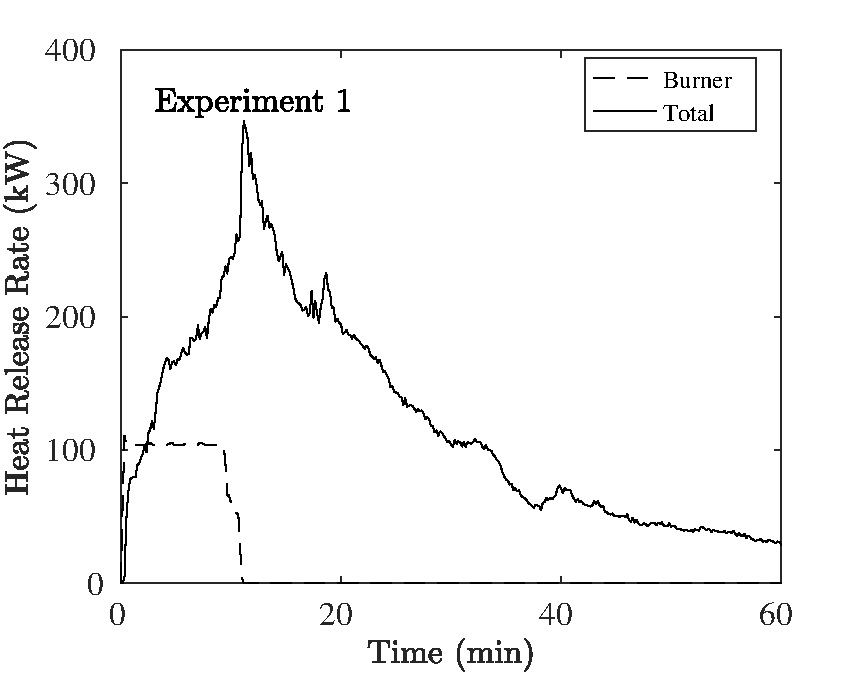
\includegraphics[height=2.15in]{../SCRIPT_FIGURES/Test_1_HRR} &
\includegraphics[height=2.15in]{../SCRIPT_FIGURES/Test_1_Gases} \\
\multicolumn{2}{c}{\includegraphics[width=\textwidth]{../FIGURES/Test_1_photo.jpg}}
\end{tabular*}
\caption{Heat release rate and gas concentrations for Test~1.}
\label{fig:Test_1}
\end{figure}


\newpage

\subsection{Test 2}

This was a repeat of Test~1. The opened panel on the right side was secured, but some noticeable opening still occurred. The HRR reached approximately 400~kW and the oxygen concentration dropped to zero.

\begin{figure}[!h]
\begin{tabular*}{\textwidth}{l@{\extracolsep{\fill}}r}
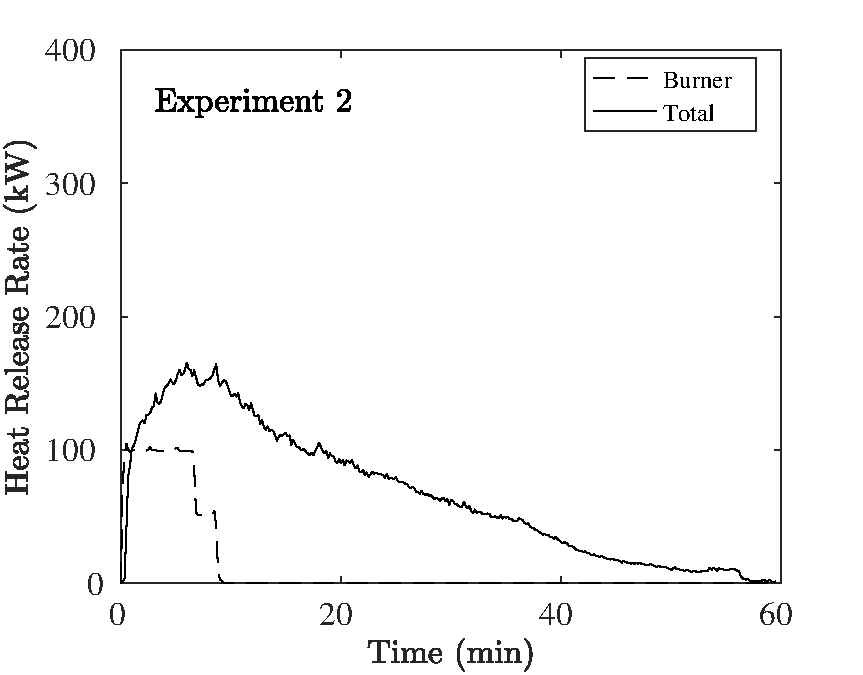
\includegraphics[height=2.15in]{../SCRIPT_FIGURES/Test_2_HRR} &
\includegraphics[height=2.15in]{../SCRIPT_FIGURES/Test_2_Gases} \\
\multicolumn{2}{c}{\includegraphics[width=\textwidth]{../FIGURES/Test_2_photo.jpg}}
\end{tabular*}
\caption{Heat release rate and gas concentrations for Test~2.}
\label{fig:Test_2}
\end{figure}


\newpage

\subsection{Test 3}

The right side vents of Enclosure~\#5 were closed using mineral wool and steel plates as shown in Fig.~\ref{Test_3}. The burner remained in the front of the right enclosure. The HRR reached approximately 160~kW and the oxygen concentration dropped to nearly zero.

\begin{figure}[!h]
\begin{tabular*}{\textwidth}{l@{\extracolsep{\fill}}r}
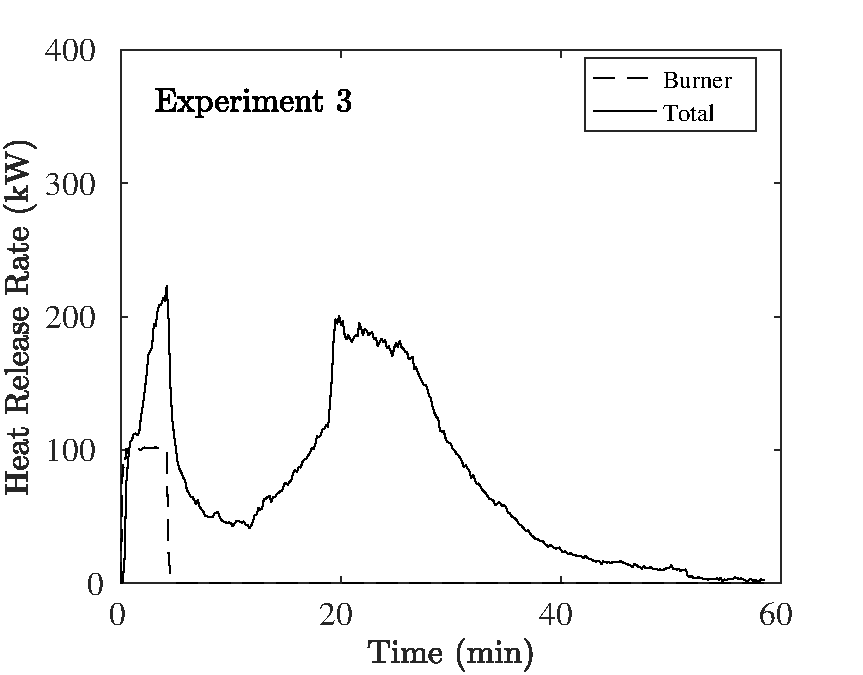
\includegraphics[height=2.15in]{../SCRIPT_FIGURES/Test_3_HRR} &
\includegraphics[height=2.15in]{../SCRIPT_FIGURES/Test_3_Gases} \\
\multicolumn{2}{c}{\includegraphics[width=\textwidth]{../FIGURES/Test_3_photo.jpg}}
\end{tabular*}
\caption{Heat release rate and gas concentrations for Test~3.}
\label{fig:Test_3}
\end{figure}


\end{document}
